\section{The Pairing model}

The Pairing model hamiltonian, when limited to up to two-body interactions, is defined as:

\begin{equation}
  \hat{H} = \sum_{\alpha\beta} \bra{\alpha}h_0\ket{\beta}\hc{a}{\alpha}\op{a}{\beta} + \frac{1}{4} \sum_{\alpha\beta\gamma\delta} \bra{\alpha\beta}\hat{V}\ket{\gamma\delta} \hc{a}{\alpha}\hc{a}{\beta}\op{a}{\delta}\op{a}{\gamma}
  \label{eq:Pairing_model_theory}
\end{equation}

The hamiltonian represents fermions in a 

With the assumption that the single particle energies grows linearly with the single particle levels $(p - 1)$ and that the two-body interaction strength is constant, we define

\begin{equation}
  \begin{gathered}
    \hat{H}_0 = \epsilon \sum_{p\sigma} \left(p - 1\right) \hc{a}{p\sigma} \op{a}{p\sigma} \\
    \hat{V} = -\frac{1}{2}g\sum_{pq} \hc{a}{p+}\hc{a}{p-}\op{a}{q-}\op{a}{q+} \; ,
  \end{gathered}
  \label{eq:sub_hamiltonian_pairing_imp}
\end{equation}

where $\epsilon$ defines the energy gap between levels, and $g$ represents the two-body pairing contribution strength. We will focus on the case of $S=0$, which means the system contains no broken pairs. If we then define the creation and annihilation operators for a pair

\begin{equation*}
  \begin{gathered}
    \hat{P}_p^+ = \hc{a}{p+}\hc{a}{p-}\\
    \hat{P}_p^- = \op{a}{p-}\op{a}{p+} \; ,
  \end{gathered}
\end{equation*}

  we can rewrite the hamiltonian as

\begin{equation}
  \hat{H} = \epsilon \sum_{p\sigma} \left(p-1\right)\hc{a}{p\sigma}\op{a}{p\sigma} - \frac{1}{2}g\sum_{pq}\hat{P}_p^+\hat{P}_q^- \; .
  \label{eq:Pairing_model_final}
\end{equation}

If we further think of pairs of particles as a particle in and of itself instead, we can rewrite it again:

$$\hat{H} = 2\varepsilon \sum_p \hc{a}{p}\op{a}{p} - \frac{1}{2}g\sum_{pq} \hc{a}{p}\op{a}{q} \; .$$

With this we can take a look at a state

$$\ket{\psi} = \ket{\alpha_{1}\alpha_{2}\dots\alpha_{P}} \;,$$

where $P$ is the number of included energy levels in our model. In the light of constructing the Hamiltonian matrix we can view the set $\{\alpha_1, \alpha_2, \dots, \alpha_P \}$ representing that a pair of particles is occupying energy level $i$ if $\alpha_i = 1$ and that it is empty if $\alpha_i = 0$. If we then apply the Hamiltonian to the state:

$$\hat{H} \ket{\psi} = \hat{H_0} \ket{\psi} + \hat{H_1} \ket{\psi} \;, $$

where we first look at the single particle contributions. The single particle energy only comes into account when $\hc{a}{p}\op{a}{p}$ encounters a pair at a energy level, and then it contributes with a factor of $(p-1)$. In our state we have already encoded the layer count into each $\alpha$, which means that for the case where $\alpha_i = 1$ we will see a contribution of $(i-1)$. We can then add together each $i$ where $\alpha_i = 1$ and then subtract the number of pairs we have in our model to get the whole single particle contribution. 

When it comes to the pair excitation part, $H_1$, we only see a contribution where a state differs from $\ket{\psi}$ by two quantum numbers $\alpha$. As an example we will look at the two-layered Pairing model with one pair.

$$\mathbf{H} = \begin{bmatrix}
\bra{00} H \ket{00} & \bra{00} H \ket{10} &\bra{00} H \ket{01} & \bra{00} H \ket{11} \\
\bra{10} H \ket{00} & \bra{10} H \ket{10} &\bra{10} H \ket{01} & \bra{10} H \ket{11} \\
\bra{01} H \ket{00} & \bra{01} H \ket{10} &\bra{01} H \ket{01} & \bra{01} H \ket{11} \\
\bra{11} H \ket{00} & \bra{11} H \ket{10} &\bra{11} H \ket{01} & \bra{11} H \ket{11} \\
\end{bmatrix} \; ,
$$

The states $\ket{00}$ and $\ket{11}$ cannot be created through our Hamiltonian \ref{eq:Pairing_model_final} because we can only move pairs, not create or destroy them, so we can safely say that 

$$ H \ket{00} = H\ket{11} = 0$$

 We then have only the block of four in the middle, and starting with $\bra{10}H\ket{10}$. For the single particle part we have: 

 $$H_0 \ket{10} = 2\varepsilon\left[(1-1)\hc{a}{1}\op{a}{1}\ket{10} + (2-1)\hc{a}{2}\op{a}{2}\ket{10}\right] = 0\; ,$$

 and

 
 $$H_0 \ket{01} = 2\varepsilon\left[(1-1)\hc{a}{1}\op{a}{1}\ket{01} + (2-1)\hc{a}{2}\op{a}{2}\ket{01} \right]=2\varepsilon\ket{01} \; ,$$
 
For the $H_1$ we have the matrix elements we have the contributions 

\begin{align*}
H_1\ket{10} &= -\frac{1}{2}g\left ( \hc{a}{1}\op{a}{2} \ket{10} + \hc{a}{2}\op{a}{1}\ket{10} \right) \\
            &=-\frac{1}{2}g \ket{01} \; .
\end{align*}

For $\ket{01}$ we then have

\begin{align*} 
H_1\ket{01} &= -\frac{1}{2}g\left ( \hc{a}{1}\op{a}{2} \ket{01} + \hc{a}{2}\op{a}{1}\ket{01} \right) \\
            &=-\frac{1}{2}g \ket{10} \; .
\end{align*}

And summarized we have that

$$\hat{H} \ket{10} =-\frac{1}{2}g \ket{01}$$
$$\hat{H} \ket{01} = 2\varepsilon\ket{01} - \frac{1}{2}g\ket{10}$$

This give us then the matrix elements:

\begin{align*}
  \bra{10}\hat{H} \ket{10} &= 0\\
  \bra{10}\hat{H} \ket{01} &= -\frac{1}{2}g\\
  \bra{01}\hat{H} \ket{01} &= 2\varepsilon\\
  \bra{01}\hat{H} \ket{10} &= -\frac{1}{2}g\\
\end{align*}

and we can get the the whole Hamiltonian matrix:

$$\mathbf{H} = \begin{bmatrix}
  0 & 0 & 0 & 0 \\
  0 & 0 & -\frac{1}{2}g & 0 \\
  0 & -\frac{1}{2}g & 2\varepsilon & 0 \\
  0 & 0 & 0 & 0 \\
\end{bmatrix} \; ,
$$

\subsection{Eigenvalues by diagonalization}

Diagonalizing the above matrix with a $\varepsilon = 0.5$ and varying $g=-1 \rightarrow g=1$ we get:
\begin{figure}[H]
  \begin{center}
    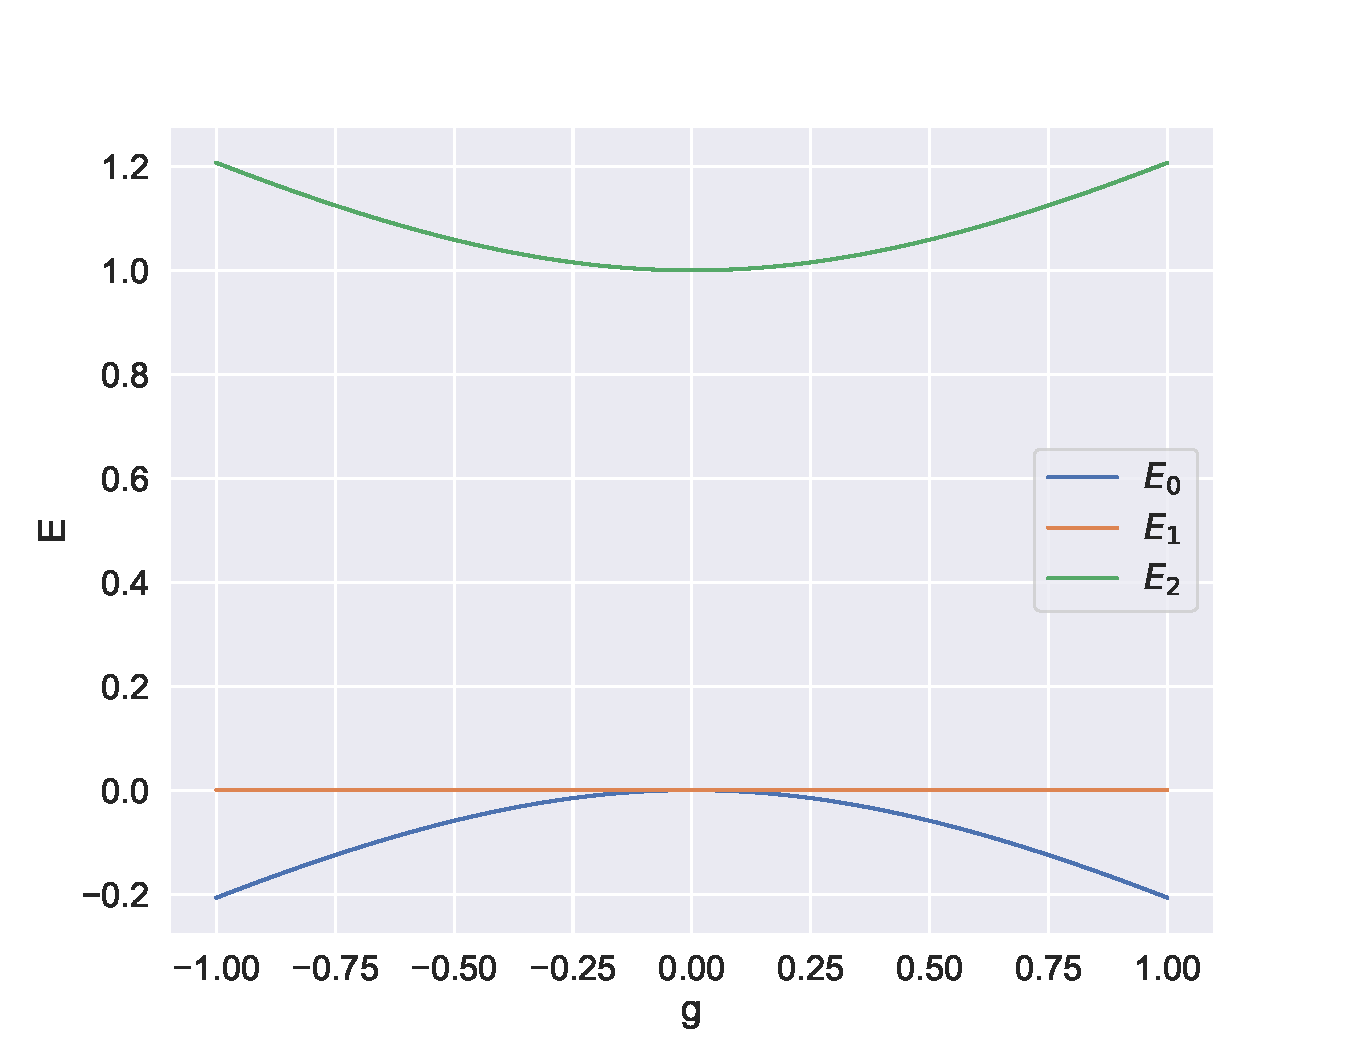
\includegraphics[width=0.95\textwidth]{Figures/Plots/Pairing/pairing_eps05_P2N1}
  \end{center}
  \caption{The Pairing model with $P = 2$ and $n=1$ where we have set $\varepsilon = 0.5$. Eigenvalues of the Hamiltnian matrix computed through diagonalization.}
\end{figure}
For a system where we include three energy levels, continuing with one pair, and changing we get:

\begin{figure}[H]
  \begin{center}
    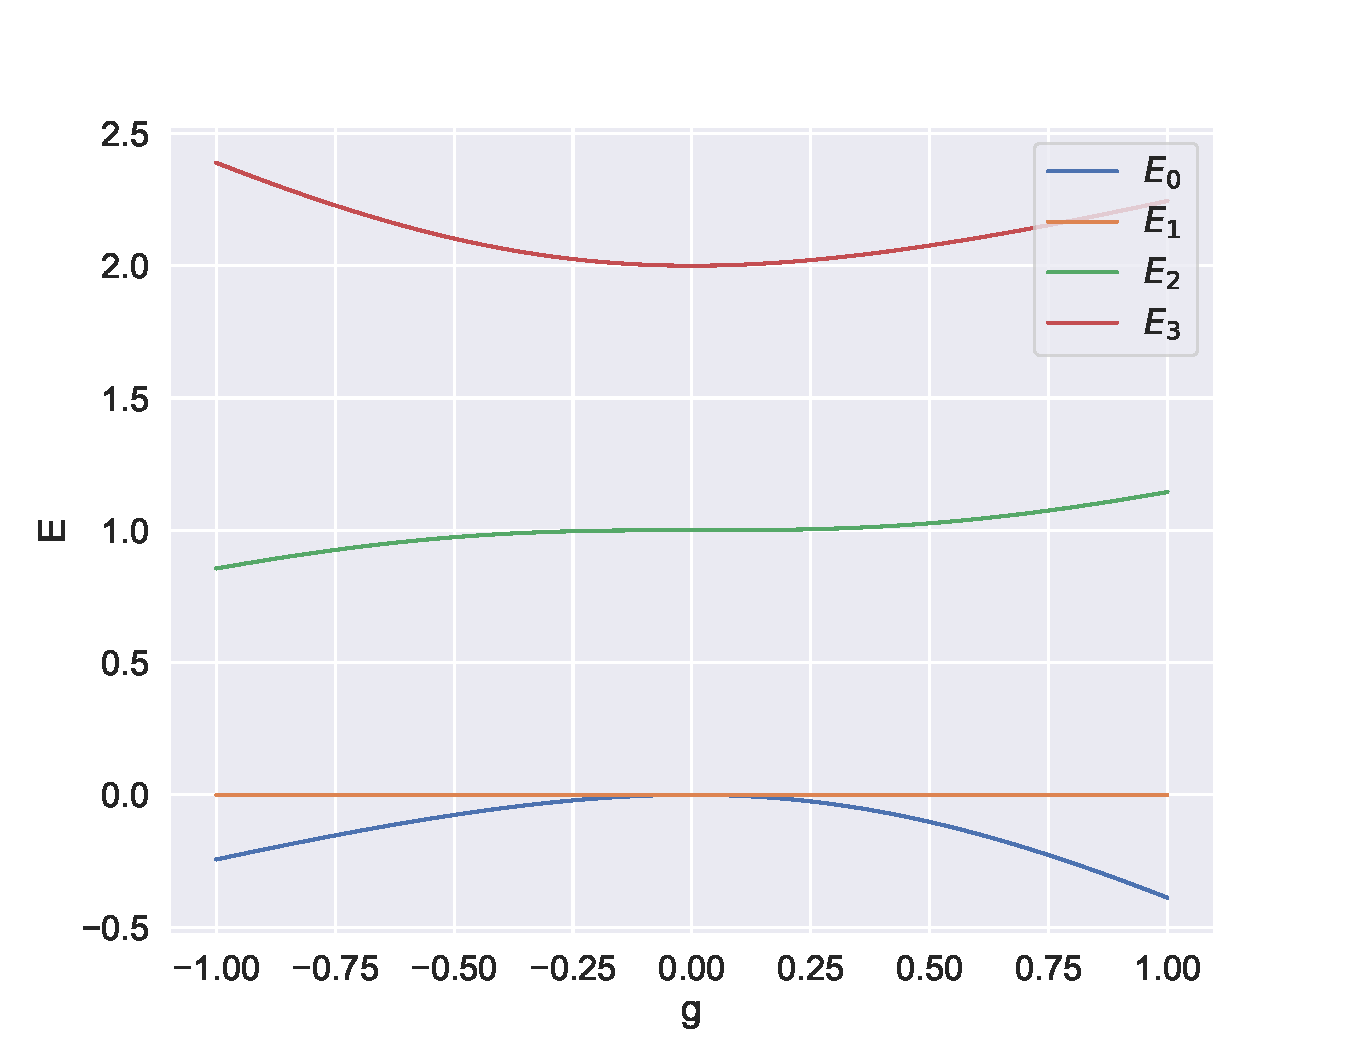
\includegraphics[width=0.95\textwidth]{Figures/Plots/Pairing/pairing_eps05_P3N1}
  \end{center}
  \caption{The Pairing model with $P = 3$ and $n=1$ where we have set $\varepsilon = 0.5$. Eigenvalues of the Hamiltnian matrix computed through diagonalization.}
\end{figure}



